\chapter{Introduction to Symmetry}

\section{Intuition and Motivation}

The idea of symmetry is the the object has a property that remains invariant under a transformation. For example, if we rotate a square by 90 degrees, the square remains the same. However, symmetry is more than a geometric concept. It is a fundamental concept in mathematics and physics.

\begin{example}[Polygons]
    We can rotate the following triangle with respect to $O$ by $120^{\circ}$, and the triangle remains the same. This triangle has rotational symmetry. 

    \begin{center}
        \begin{tikzpicture}[baseline=(current bounding box.center)]
            % A regular triangle with a dot in the center
            \draw (0, 0) -- (2, 0) -- (1, 1.732) -- cycle;

            % The center of the triangle
            \node[graph-node, label=above:$O$] at (1, 0.577) {};

            % The labels of the vertices
            \node[below] at (0, 0) {$B$};
            \node[below] at (2, 0) {$C$};
            \node[above] at (1, 1.732) {$A$};
        \end{tikzpicture}%
        \hfil$\xrightarrow{\text{rotate by } 120^{\circ}}$\hfil
        \begin{tikzpicture}[baseline=(current bounding box.center)]
            % A regular triangle with a dot in the center
            \draw (0, 0) -- (2, 0) -- (1, 1.732) -- cycle;

            % The center of the triangle
            \node[graph-node, label=above:$O$] at (1, 0.577) {};

            % The labels of the vertices
            \node[below] at (0, 0) {$A$};
            \node[below] at (2, 0) {$B$};
            \node[above] at (1, 1.732) {$C$};
        \end{tikzpicture}
    \end{center}

    Moreover, we can also reflect the triangle with respect to the line $l$ passing through $O$, and the triangle remains the same. This triangle has reflection symmetry.

    \begin{center}
        \begin{tikzpicture}[baseline=(current bounding box.center)]
            % A regular triangle with a dot in the center
            \draw (0, 0) -- (2, 0) -- (1, 1.732) -- cycle;

            % The center of the triangle
            \node[graph-node, label=above:$O$] at (1, 0.577) {};

            % The labels of the vertices
            \node[below] at (0, 0) {$B$};
            \node[below] at (2, 0) {$C$};
            \node[above] at (1, 1.732) {$A$};

            % The line l with the label
            \draw[dashed] (1, 2.5) -- (1, -0.5);
            \node[below] at (1, -0.5) {$l$};
        \end{tikzpicture}%
        \hfil$\xrightarrow{\text{reflect with respect to } l}$\hfil
        \begin{tikzpicture}[baseline=(current bounding box.center)]
            % A regular triangle with a dot in the center
            \draw (0, 0) -- (2, 0) -- (1, 1.732) -- cycle;

            % The center of the triangle
            \node[graph-node, label=above:$O$] at (1, 0.577) {};

            % The labels of the vertices
            \node[below] at (0, 0) {$C$};
            \node[below] at (2, 0) {$B$};
            \node[above] at (1, 1.732) {$A$};
        \end{tikzpicture}
    \end{center}

    Is there any other symmetry? Yes, we can combine the two symmetries above. We first rotate the triangle by $120^{\circ}$, and then reflect it with respect to $l$. This triangle has both rotational and reflection symmetry.

    % Graph of the triangle
    \begin{center}
        \begin{tikzpicture}[baseline=(current bounding box.center)]
            % A regular triangle with a dot in the center
            \draw (0, 0) -- (2, 0) -- (1, 1.732) -- cycle;

            % The center of the triangle
            \node[graph-node, label=above:$O$] at (1, 0.577) {};

            % The labels of the vertices
            \node[below] at (0, 0) {$B$};
            \node[below] at (2, 0) {$C$};
            \node[above] at (1, 1.732) {$A$};
        \end{tikzpicture}%
        \hfil$\xrightarrow{\text{rotate by } 120^{\circ}}$\hfil
        \begin{tikzpicture}[baseline=(current bounding box.center)]
            % A regular triangle with a dot in the center
            \draw (0, 0) -- (2, 0) -- (1, 1.732) -- cycle;

            % The center of the triangle
            \node[graph-node, label=above:$O$] at (1, 0.577) {};

            % The labels of the vertices
            \node[below] at (0, 0) {$A$};
            \node[below] at (2, 0) {$B$};
            \node[above] at (1, 1.732) {$C$};

            % The line l with the label
            \draw[dashed] (1, 2.5) -- (1, -0.5);
            \node[below] at (1, -0.5) {$l$};
        \end{tikzpicture}%
        \hfil$\xrightarrow{\text{reflect with respect to } l}$\hfil
        \begin{tikzpicture}[baseline=(current bounding box.center)]
            % A regular triangle with a dot in the center
            \draw (0, 0) -- (2, 0) -- (1, 1.732) -- cycle;

            % The center of the triangle
            \node[graph-node, label=above:$O$] at (1, 0.577) {};

            % The labels of the vertices
            \node[below] at (0, 0) {$B$};
            \node[below] at (2, 0) {$A$};
            \node[above] at (1, 1.732) {$C$};
        \end{tikzpicture}
    \end{center}
\end{example}

The above example is a very simple one. However, given an general object, it is not easy to find all its symmetries. We can label the vertices of the triangle with $A, B, C$, then permute the labels. 

\begin{center}
    \begin{tikzpicture}[baseline=(current bounding box.center)]
        % A regular triangle with a dot in the center
        \draw (0, 0) -- (2, 0) -- (1, 1.732) -- cycle;

        % The center of the triangle
        \node[graph-node, label=above:$O$] at (1, 0.577) {};

        % The labels of the vertices
        \node[draw,fill=white,circle] at (0, 0) {?};
        \node[draw,fill=white,circle] at (2, 0) {?};
        \node[draw,fill=white,circle] at (1, 1.732) {?};
    \end{tikzpicture}
\end{center}

Since the transformations are linear, they preserve linearity. This, it suffices to consider the transformations of the vertices. 

\begin{example}[Continued]
    The following table shows all the permutations of the vertices of the triangle. 

    \begin{table}[ht!]
        \centering
        \begin{tabular}{|c|c|c|c|}
            \hline
            Identity & $A$ & $B$ & $C$ \\
            \hline
            Rotation & $C$ & $A$ & $B$ \\
            \hline
            Reflection & $A$ & $C$ & $B$ \\
            \hline
            Rotation + Reflection & $C$ & $B$ & $A$ \\
            \hline \hline
            & $B$ & $A$ & $C$ \\
            \hline
            & $B$ & $C$ & $A$ \\
            \hline
        \end{tabular}
    \end{table}

    As we can see, there are six transformations of the vertices, each of which corresponds to a symmetry of the triangle. 
\end{example}

Naively, given an square, one would argue that there are $24$ ways to permute the vertices, and thus $24$ symmetries. However, this is not true. There are certain permutations that are not symmetries. 

\begin{center}
    \begin{tikzpicture}[baseline=(current bounding box.center)]
        % The square
        \draw (0, 0) -- (1, 0) -- (1, 1) -- (0, 1) -- cycle;

        % The labels of the vertices
        \node[below] at (0, 0) {$A$};
        \node[right] at (1, 0) {$B$};
        \node[above] at (1, 1) {$C$};
        \node[left] at (0, 1) {$D$};
    \end{tikzpicture}
    $\xrightarrow{\text{swap } A \text{ and } B}$
    \begin{tikzpicture}[baseline=(current bounding box.center)]
        % The square
        \draw (0, 0) -- (1, 0) -- (1, 1) -- (0, 1) -- cycle;

        % The labels of the vertices
        \node[below] at (0, 0) {$B$};
        \node[right] at (1, 0) {$A$};
        \node[above] at (1, 1) {$C$};
        \node[left] at (0, 1) {$D$};
    \end{tikzpicture}
\end{center}

\section{Symmetric Group}

\begin{definition}[Symmetric Group]\index{Symmetric Group}\label{def:symmetric_group}
    The \term{symmetric group}, denoted $S_n$, is the set of all permutations of $n$ elements $1, 2, \dots, n$.
\end{definition}

\begin{definition}[Identity Permutation]\index{Identity Permutation}\label{def:identity_permutation}
    The \term{identity permutation} is the permutation that does not change the order of the elements.
\end{definition}

\begin{example}
    The identity permutation of $S_3$ is the identity permutation of $1, 2, 3$.
\end{example}

\begin{definition}[Transposition]\index{Transposition}\label{def:transposition}
    A \term{transposition} is a permutation that swaps two elements and leaves the other elements unchanged.
\end{definition}

\begin{example}
    The following are some transpositions of $S_3$.
    \begin{itemize}
        \item $2, 1, 3$ swaps $1$ and $2$.
        \item $1, 3, 2$ swaps $2$ and $3$.
        \item $3, 2, 1$ swaps $1$ and $3$.
    \end{itemize}
\end{example}

\begin{definition}[Cycle]\index{Cycle}\label{def:cycle}
    A \term{cycle} is a permutation that moves the first element to the second, the second to the third, and so on, and the last element to the first.
\end{definition}

\begin{example}
    The cycle $3, 2, 1$ moves $1$ to $3$, $3$ to $2$, and $2$ to $1$.
\end{example}

\begin{definition}[Permutation]\index{Permutation}\label{def:permutation}
    A \text{permutation} is a way to order $n$ elements. We codify them in ``cycles''
\end{definition}

\begin{example}
    Consider $S_3$. 

    \begin{table}[ht!]
        \centering
        \begin{tabular}{c c c c c c}
            1 2 3 & 1 2 3 & 1 2 3 & 1 2 3 & 1 2 3 & 1 2 3 \\
            \hline 
            1 2 3 & 1 3 2 & 3 2 1 & 2 1 3 & 3 1 2 & 2 3 1 \\
            (1)(2)(3) & (1)(23) & (13)(2) & (12)(3) & (132) & (123) \\
        \end{tabular}
    \end{table}

    Here, $(1)(23)$ means

    \begin{itemize}
        \item $1$ goes to $1$.
        \item $2$ goes to $3$, and $3$ goes to $2$.
    \end{itemize}
\end{example}

\begin{example}
    Consider the following permutation. 

    \begin{table}[ht!]
        \centering
        \begin{tabular}{c|c}
            1 2 3 4 5 6 7 & 1 2 3 4 5 6 7 \\
            \hline
            3 4 2 1 7 5 6 & \color{blue}2 3 1 4 6 5 7 \\
            \color{blue}(1324)(576) & (1 2 3)(5 6)
        \end{tabular}
    \end{table}
\end{example}

\begin{example}
    Suppose you have two permutations $\sigma$ and $\tau$:

    \begin{listu}
        \item $\sigma = (1 2)(3 4 5 6)$
        \item $\tau = (1 6 5 4)(3 2)$
    \end{listu}

    What happens if we perform one after the other?

    \begin{listu}
        \item $\sigma$ first, $\tau$ second\footnote{Note that we read from right to left.}: $\color{red}(1 6 5 4)(3 2) \color{blue}(1 2)(3 4 5 6) \color{black} = (1 6 5 4)(3 2)(1 2)(3 4 5 6)$

        \begin{listu}
            \item We start with $1$: $1 \to 2 \to 3$, so $1 \to 3$. 
            \item We then consider $3$: $3 \to 4 \to 1$, so $3 \to 1$.
            \item Now, we consider $2$: $2 \to 1 \to 6$, so $2 \to 6$.
            \item $6 \to 3 \to 2$, so $6 \to 2$.
            \item $4 \to 5 \to 4$, so $4 \to 4$.
            \item $5 \to 6 \to 5$, so $5 \to 5$.
        \end{listu}

        Thus, we get \[(1 3)(2 6)(4)(5). \]

        \item $\tau$ first, $\sigma$ second: $\color{red}(1 2)(3 4 5 6) \color{blue}(1 6 5 4)(3 2) \color{black} = (1 2)(3 4 5 6)(1 6 5 4)(3 2)$

        \begin{listu}
            \item We start with $1$: $1 \to 6 \to 4$, so $1 \to 3$. 
            \item We then consider $3$: $4 \to 5 \to 1$, so $4 \to 1$.
            \item \dots
        \end{listu}

        Eventually, we get \[(1 3)(2 4)(5)(6). \]
    \end{listu}
        
    It is important to note that the order of the permutations matters.
\end{example}

The above example demonstrates an important property of permutations: closed under composition. That is, if we ``merge'' two permutations, we get another permutation.

\newpage
\begin{table}[ht!]
    \centering
    \renewcommand{\arraystretch}{1.25}
    \begin{tabular}{c|c|c|c|c|c|c}
        $\circ$ & $\mathds{1}$ & (12) & (13) & (23) & (123) & (132) \\
        \hline
        $\mathds{1}$ & & & & & \\
        \hline
        $(12)$ & & & & & \\
        \hline
        $(13)$ & & & & & \\
        \hline
        $(23)$ & (23) & (132) & (123) & $\mathds{1}$ & (13) & (12)\\
        \hline
        $(123)$ & & & & & \\
        \hline
        $(132)$ & & & & &
    \end{tabular}
\end{table}

This is a multiplication table of $S_3$. Symmetries of the same group have the same multiplication table, despite the fact that they are different permutations.

\begin{remark}
    Note that in the above table of $S_3$, we have $(1 2 3) = (2 3)(1 3)$, and $(1 3 2) = (2 3)(1 2)$. \bred{All the permutations can be written as a composition of transpositions.} 

    It is important to note that this is not unique. For example, we can write $\mathds{1} = (12)(12)$. 
\end{remark}

\begin{theorem}
    The amount of transpositions needed to create a permutation preservers its parity.
\end{theorem}

In other words, if a permutation $\alpha$ can be expressed as a product of transpositions \[
    \alpha = \tau_1 \tau_2 \dots \tau_n \qquad \text{ and } \qquad \alpha = \sigma_1 \sigma_2 \dots \sigma_m
\] where $\tau$ and $\sigma$ are transpositions, then $n$ and $m$ have the same parity (both even or both odd). The smaller groups are called \term{alternating groups}.

\begin{example}
    Consider the following figure of a cube.

    % TODO: figure
    \begin{center}
        \begin{tikzpicture}
            % Coordinates of the vertices
            \coordinate (A) at (0, 0);
            \coordinate (B) at (0, 2);
            \coordinate (C) at (2, 2);
            \coordinate (D) at (2, 0);
            \coordinate (E) at (0.5, 0.5);
            \coordinate (F) at (0.5, 2.5);
            \coordinate (G) at (2.5, 2.5);
            \coordinate (H) at (2.5, 0.5);

            % The cube
            \draw (A) -- (B) -- (C) -- (D) -- cycle;
            \draw (A) -- (E) -- (F) -- (B);
            \draw (D) -- (H) -- (G) -- (C);
            \draw (E) -- (F) -- (G) -- (H) -- cycle;

            % The center of the top face
            \draw[dashed] (B) -- (G);
            \draw[dashed] (F) -- (C);
            \node[graph-node,red] at (1.25, 2.25) {};

            % The vertices
            \node[graph-node,blue]   at (A) {};
            \node[graph-node,orange] at (B) {};
            \node[graph-node,blue]   at (C) {};
            \node[graph-node,orange] at (D) {};
            \node[graph-node,orange] at (E) {};
            \node[graph-node,blue]   at (F) {};
            \node[graph-node,orange] at (G) {};
            \node[graph-node,blue]   at (H) {};

            % The label $C$
            \node[magenta] at (2, 2.25) {$C$};
        \end{tikzpicture}
    \end{center} which expands to the following graph.

    % TODO: figure
    \begin{center}
        \begin{tikzpicture}
            % The cube expanded to 2D
            \draw (0, 0) -- (0, 1) -- (1, 1) -- (1, 0) -- cycle;
            \draw (0, 0) -- (-1, 0) -- (-1, 1) -- (0, 1);
            \draw (1, 1) -- (2, 1) -- (2, 0) -- (1, 0);
            \draw (2, 1) -- (3, 1) -- (3, 0) -- (2, 0);
            \draw (0, 1) -- (0, 2) -- (1, 2) -- (1, 1);
            \draw (1, 0) -- (1, -1) -- (0, -1) -- (0, 0);

            % Crosses on the cube
            \draw[dashed] (-1, 1) -- (0, 0) -- (1, 1) -- (2, 0) -- (3, 1);
            \draw[dashed] (-1, 0) -- (0, 1) -- (1, 0) -- (2, 1) -- (3, 0);
            \draw[dashed] (0, 2) -- (1, 1);
            \draw[dashed] (0, 1) -- (1, 2);
            \draw[dashed] (0, -1) -- (1, 0);
            \draw[dashed] (0, 0) -- (1, -1);

            % The vertices
            \node[graph-node,blue]   at (-1, 0) {};
            \node[graph-node,orange] at (-1, 1) {};
            \node[graph-node,orange] at (0, 0) {};
            \node[graph-node,blue]   at (0, 1) {};
            \node[graph-node,orange] at (1, 1) {};
            \node[graph-node,blue]   at (1, 0) {};
            \node[graph-node,orange] at (0, 2) {};
            \node[graph-node,blue]   at (1, 2) {};
            \node[graph-node,orange] at (1, -1) {};
            \node[graph-node,blue]   at (0, -1) {};
            \node[graph-node,blue]   at (2, 1) {};
            \node[graph-node,orange] at (2, 0) {};
            \node[graph-node,orange] at (3, 1) {};
            \node[graph-node,blue]   at (3, 0) {};

            % The centers of the crosses
            \node[graph-node,red] at (-0.5, 0.5) {};
            \node[graph-node,red] at (0.5, 0.5) {};
            \node[graph-node,red] at (0.5, 0.5) {};
            \node[graph-node,red] at (0.5, 1.5) {};
            \node[graph-node,red] at (0.5, -0.5) {};
            \node[graph-node,red] at (1.5, 0.5) {};
            \node[graph-node,red] at (2.5, 0.5) {};

            % The label $C$
            \node[right,magenta] at (0.5, 0.5) {$C$};
        \end{tikzpicture}
    \end{center}

    \textbf{Question}: What are the isometries that preserve the colouring of this object?

    \begin{definition}[Isometry]\index{Isometry}\label{def:isometry}
        An \term{isometry} is a transformation that preserves distance.
    \end{definition}

    \begin{remark}
        Consider reflection with respect to the planes $\sigma_1$, $\sigma_2$, and $\sigma_3$.

            \begin{center}
                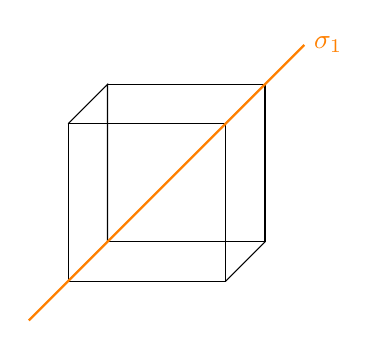
\begin{tikzpicture}[baseline=(current bounding box.south)]
                    % Coordinates of the vertices
                    \coordinate (A) at (0, 0);
                    \coordinate (B) at (0, 2);
                    \coordinate (C) at (2, 2);
                    \coordinate (D) at (2, 0);
                    \coordinate (E) at (0.5, 0.5);
                    \coordinate (F) at (0.5, 2.5);
                    \coordinate (G) at (2.5, 2.5);
                    \coordinate (H) at (2.5, 0.5);

                    % The cube
                    \draw (A) -- (B) -- (C) -- (D) -- cycle;
                    \draw (A) -- (E) -- (F) -- (B);
                    \draw (D) -- (H) -- (G) -- (C);
                    \draw (E) -- (F) -- (G) -- (H) -- cycle;

                    % The plane
                    \draw[thick,orange] (-0.5, -0.5) -- (3, 3);
                    \node[orange,right] at (3, 3) {$\sigma_1$};
                \end{tikzpicture}
                \hfil%
                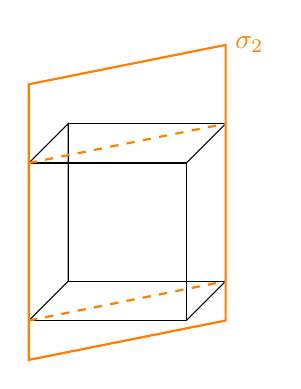
\begin{tikzpicture}[baseline=(current bounding box.south)]
                    % Coordinates of the vertices
                    \coordinate (A) at (0, 0);
                    \coordinate (B) at (0, 2);
                    \coordinate (C) at (2, 2);
                    \coordinate (D) at (2, 0);
                    \coordinate (E) at (0.5, 0.5);
                    \coordinate (F) at (0.5, 2.5);
                    \coordinate (G) at (2.5, 2.5);
                    \coordinate (H) at (2.5, 0.5);

                    % The cube
                    \draw (A) -- (B) -- (C) -- (D) -- cycle;
                    \draw (A) -- (E) -- (F) -- (B);
                    \draw (D) -- (H) -- (G) -- (C);
                    \draw (E) -- (F) -- (G) -- (H) -- cycle;

                    % The plane
                    \draw[thick,orange] (0, -0.5) -- (0, 3) -- (2.5, 3.5) -- (2.5, 0) -- cycle;
                    \draw[thick,dashed,orange] (A) -- (H);
                    \draw[thick,dashed,orange] (B) -- (G);
                    \node[orange,right] at (2.5, 3.5) {$\sigma_2$};
                \end{tikzpicture}
                \hfil
                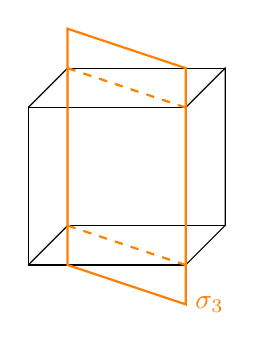
\begin{tikzpicture}[baseline=(current bounding box.south)]
                    % Coordinates of the vertices
                    \coordinate (A) at (0, 0);
                    \coordinate (B) at (0, 2);
                    \coordinate (C) at (2, 2);
                    \coordinate (D) at (2, 0);
                    \coordinate (E) at (0.5, 0.5);
                    \coordinate (F) at (0.5, 2.5);
                    \coordinate (G) at (2.5, 2.5);
                    \coordinate (H) at (2.5, 0.5);

                    % The cube
                    \draw (A) -- (B) -- (C) -- (D) -- cycle;
                    \draw (A) -- (E) -- (F) -- (B);
                    \draw (D) -- (H) -- (G) -- (C);
                    \draw (E) -- (F) -- (G) -- (H) -- cycle;

                    % The plane
                    \draw[thick,orange] (0.5, 3) -- (2, 2.5) -- (2, -0.5) -- (0.5, 0) -- cycle;
                    \draw[thick,dashed,orange] (C) -- (F);
                    \draw[thick,dashed,orange] (D) -- (E);
                    \node[orange,right] at (2, -0.5) {$\sigma_3$};
                \end{tikzpicture}
            \end{center}

            % TODO: graphs of $\sigma_1$, $\sigma_2$, and $\sigma_3$. 
    \end{remark}

    \begin{center}
        \begin{tikzpicture}
            % The cube expanded to 2D
            \draw (0, 0) -- (0, 2) -- (2, 2) -- (2, 0) -- cycle;
            \draw (0, 0) -- (-2, 0) -- (-2, 2) -- (0, 2);
            \draw (2, 2) -- (4, 2) -- (4, 0) -- (2, 0);
            \draw (4, 2) -- (6, 2) -- (6, 0) -- (4, 0);
            \draw (0, 2) -- (0, 4) -- (2, 4) -- (2, 2);
            \draw (2, 0) -- (2, -2) -- (0, -2) -- (0, 0);

            % Crosses on the cube
            \draw[dashed] (-2, 2) -- (0, 0) -- (2, 2) -- (4, 0) -- (6, 2);
            \draw[dashed] (-2, 0) -- (0, 2) -- (2, 0) -- (4, 2) -- (6, 0);
            \draw[dashed] (0, 4) -- (2, 2);
            \draw[dashed] (0, 2) -- (2, 4);
            \draw[dashed] (0, -2) -- (2, 0);
            \draw[dashed] (0, 0) -- (2, -2);

            % The vertices
            \node[graph-node,blue]   at (-2, 0) {};
            \node[graph-node,orange] at (-2, 2) {};
            \node[graph-node,orange] at (0, 0) {};
            \node[graph-node,blue]   at (0, 2) {};
            \node[graph-node,orange] at (2, 2) {};
            \node[graph-node,blue]   at (2, 0) {};
            \node[graph-node,orange] at (0, 2) {};
            \node[graph-node,blue]   at (2, 2) {};
            \node[graph-node,orange] at (2, -2) {};
            \node[graph-node,blue]   at (0, -2) {};
            \node[graph-node,blue]   at (4, 2) {};
            \node[graph-node,orange] at (4, 0) {};
            \node[graph-node,orange] at (6, 2) {};
            \node[graph-node,blue]   at (6, 0) {};

            % The centers of the crosses
            \node[graph-node,red] at (-1, 1) {};
            \node[graph-node,red] at (1, 1) {};
            \node[graph-node,red] at (1, 1) {};
            \node[graph-node,red] at (1, 3) {};
            \node[graph-node,red] at (1, -1) {};
            \node[graph-node,red] at (3, 1) {};
            \node[graph-node,red] at (5, 1) {};

            % The label $C$
            \node[magenta] at (1.5, 1) {$C$};
            \node[magenta] at (2.5, 1) {$\sigma_1C$};
            \node[magenta] at (1, 1.5) {$\sigma_2C$};
            \node[magenta] at (1, 0.5) {$\sigma_3C$};
            \node[magenta] at (0.5, 1) {$D$};
        \end{tikzpicture}
    \end{center}

    $D$ can be obtained by either $\sigma_3 \sigma_2 C$ or $\sigma_2 \sigma_3 C$. \[ \begin{matrix}
        \mathbb{R}^3 & \to & \mathbb{R}^3 & \to & \mathbb{R}^3 \\
        & \sigma_3 & & \sigma_2 & \\
        & \sigma_2 & & \sigma_3 &
    \end{matrix} \]

    Matrices are not commute, and thus these transformations may be different. We ask the questions: since $\sigma_2 \sigma_1$ and $\sigma_1 \sigma_2$ move the triangle $C$ in the same way, are they the same map?

    \begin{proposition}
        If $S, T: \mathbb{R}^3 \to \mathbb{R}^3$ preserve the coloured ube and send the triangle to the same place, then $S = T$ (as maps). 
    \end{proposition}

    \begin{proof}
        WTS $S = T$.

        \begin{remark}
            It is important that the triangle $C$ is a field of vectors. 
        \end{remark}
        Consider $o = (0, 0, \frac{1}{2})$, $b = (\frac{1}{2}, \frac{1}{2}, \frac{1}{2})$, and $y = (-\frac{1}{2}, \frac{-1}{2}, \frac{1}{2})$. 

        $Sb = Tb, So = To, Sy = Ty \implies (S - T)b = 0, (S - T)o = 0, (S - T)y = 0$.

        This implies $b$, $o$, and $y$ are in the kernel of $S - T$. 

        Moreover, $b, o, y$ are linearly independent since $\det \begin{bmatrix}
            \frac{1}{2} & 0 & -\frac{1}{2} \\
            \frac{1}{2} & 0 & -\frac{1}{2} \\
            \frac{1}{2} & \frac{1}{2} & \frac{1}{2}
        \end{bmatrix} \neq 0$.

        Thus, $\dim \ker (S - T) = 3$. Since $\dim \mathbb{R}^3 = 3$, $\ker (S - T) = \mathbb{R}^3$. Thus, $S - T = 0$.
    \end{proof}

    We can reach all 24 locations of the triangle $C$ by applying $\sigma_1$, $\sigma_2$, and $\sigma_3$ to the triangle $C$. Thus, there are 24 isometries that preserve the coloured cube. Moreover, we know that $3$ of them generates the set. It suffices to study these three isometries to understand the whole group.
\end{example}